\chapter{\label{chapter3}Implementation}

\rb{again add a short introduction for this chapter and explain which sections are coming}

The main design principle when implementing Swift into the iSDX is to change as little as \\ 
possible in both the iSDX and Swift. Utilizing their similar architecture to keep the full functionality of both the iSDX and Swift.

\section{\label{chapter3:Architecture}Architecture}

\begin{figure}[h]
\center
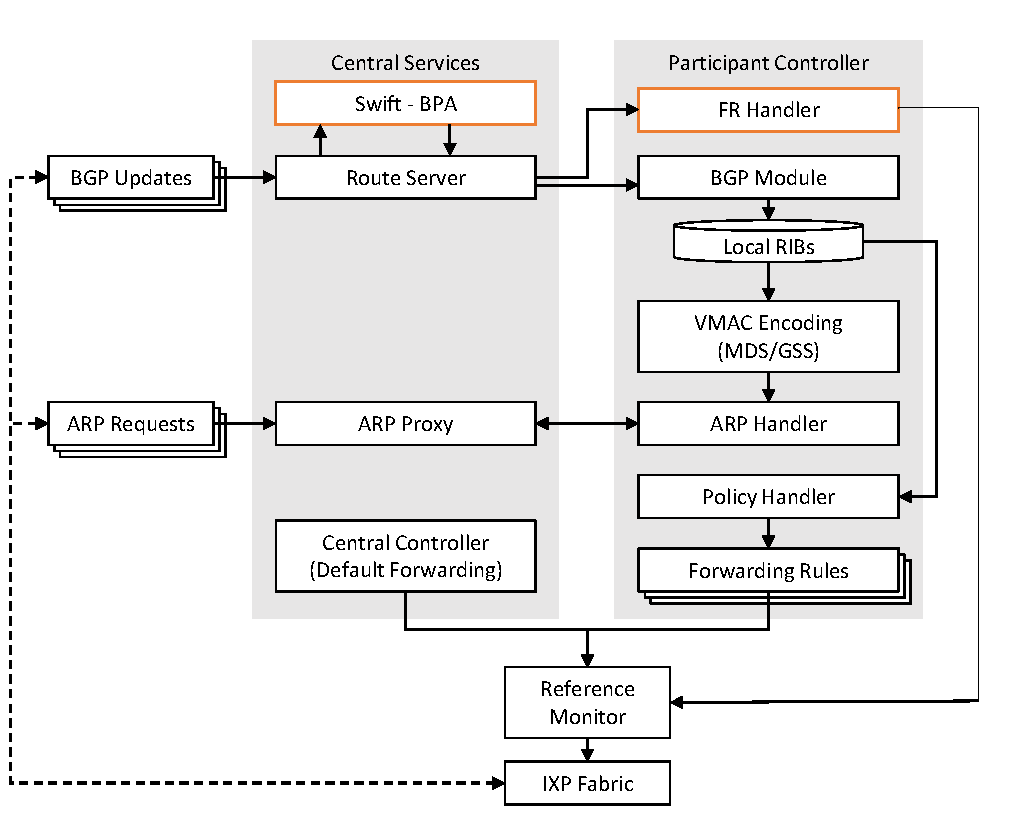
\includegraphics[scale = 0.7]{Figures/design_sdx_swift_cropped.pdf}
\caption{iSDX architecture with Swift}
\label{fig:isdx_architecture_with_swift}
\end{figure}

\rb{you can refer to figures using label and ref}
Figure~\ref{fig:isdx_architecture_with_swift} shows the iSDX architecture with Swift. The orange modules represent the new modules we had to add to the iSDX to implement Swift. The iSDX receives two additional modules the Swift-BPA module in the central services and the FR handler in the participant controller. With these two modules the iSDX will now detect bursts of withdrawals, predict the failed AS-link and push fast-reroute rules into the IXP fabric. \\
In the following sections I will go over the functionality of the new modules and other changes to the iSDX in more detail.

\section{\label{chapter3:Swift-BPA}Swift-BPA}

\begin{figure}[h]
\center
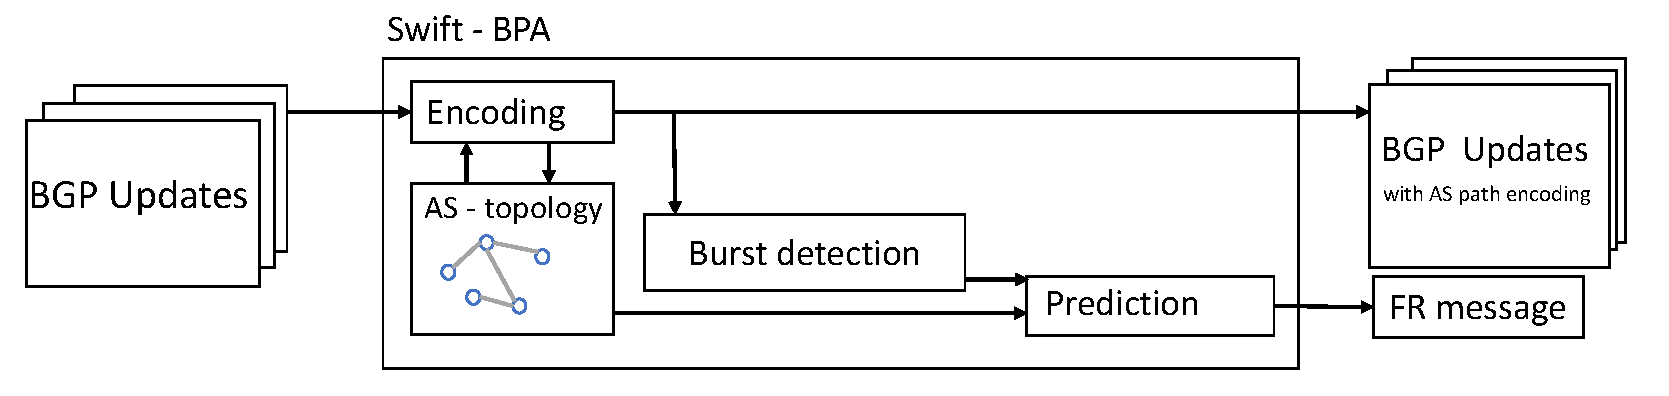
\includegraphics[scale = 0.5]{Figures/design_swift_bpa_cropped.pdf}
\caption{pipeline of the Swift-BPA module}
\end{figure}

The Swift-BPA module implements Swifts main functionality, encoding and prediction. \\
The Swift-BPA module receives BGP updates from the route server. It then adds the AS-path encoding to the BGP update and sends the modified BGP update back to the route server. \\
The Swift-BPA then checks if the received BGP updates are enough trigger a burst. If so it starts the prediction process. At the end of the prediction the Swift-BPA sends a fast-reroute message to the route server. The fast reroute message informs the participant controllers about the predicted AS-link. \\

\section{\label{chapter3:FR-handler}FR-Handler}

\begin{figure}[h]
\center
\includegraphics[scale = 0.6]{Figures/design_fr_handler_cropped.pdf}
\caption{pipeline of the fast reroute handler}
\end{figure}

The FR-handler implements the handling of FR messages and pushes fast reroute rules into the SDN switch. \\
The FR handler receives FR messages from the route server. The FR handler then computes the fast reroute rules using the backup next-hops and the predicted AS-link. The fast reroute rules get sent to the reference monitor as flow rule messages.  

\newpage

\section{\label{chapter3:Changes to the iSDX}Changes to the iSDX}

There are a few changes to the iSDX's modules. 

\paragraph{\label{chapter3:Changes to the iSDX:route server}Route Server:}

The route server now has two modules the listener and sender. \\
The listener receives BGP updates and forwards them to the Swift-BPA. \\
The sender receives modified BGP updates and FR messages from the Swift-BPA and forwards them to the participant controllers. The sender processes FR messages with higher priority than modified BGP updates, this way the FR messages reach the FR handler as quickly as possible. 

\begin{figure}[h]
\center
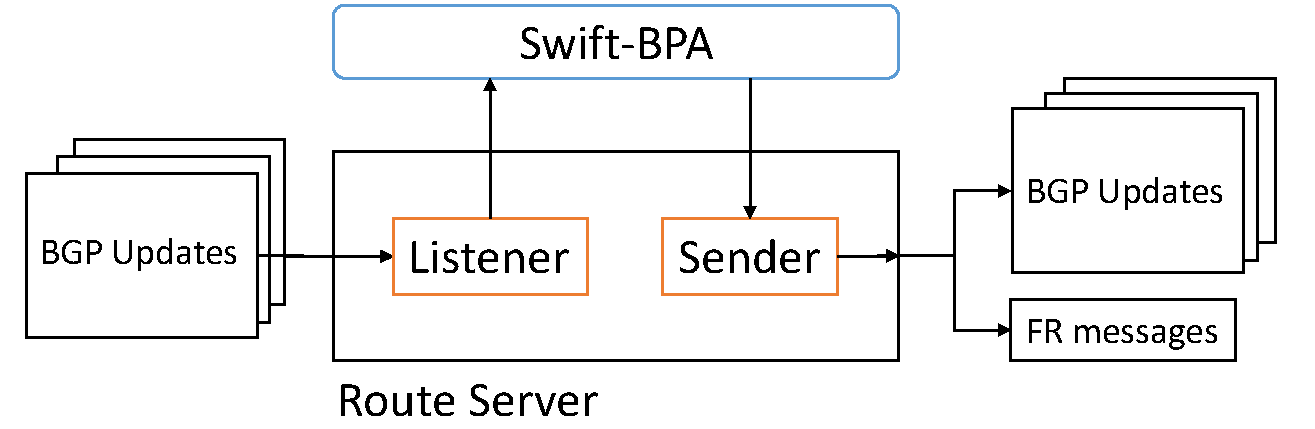
\includegraphics[scale = 0.45]{Figures/design_route_server_cropped2.pdf}
\caption{pipeline of the modified route server}
\end{figure}


\paragraph{\label{chapter3:Changes to the iSDX:local RIB}Local RIB:}
The local RIB now stores the AS-path encoding. The AS-path encoding is then used in the vmac encoding. 

\paragraph{\label{chapter3:Changes to the iSDX:Vmac Encoding}VMAC Encoding:}
The vmac encoding now computes the backup next-hops for the AS-path of the BGP update. There is one backup next-hop for every AS-link on the AS-path, packets can be sent to the backup next-hop in case this AS-link is predicted to be down. \\
The vmac encoding now builds the vmac using both iSDX and Swift encoding. \\
More in section 3.5 

\section{\label{chapter3:vmac partitioning}VMAC Partitioning}

Both Swift and the iSDX use the destination mac address to encode information about the prefix of the packet. The destination mac address has to be shared between the iSDX and the Swift encoding. This is because the iSDX and Swift encode different information about the prefix. The iSDX encodes the participants advertising the prefix and the BGP best next-hop. Swift encodes the backup next-hops and the AS-path. \\
The encoded AS-path starts with the second AS on the AS-path. This is because the first AS is already encoded as the BGP best next-hop. (in the iSDX part of the vmac)
\begin{figure}[h]
\center
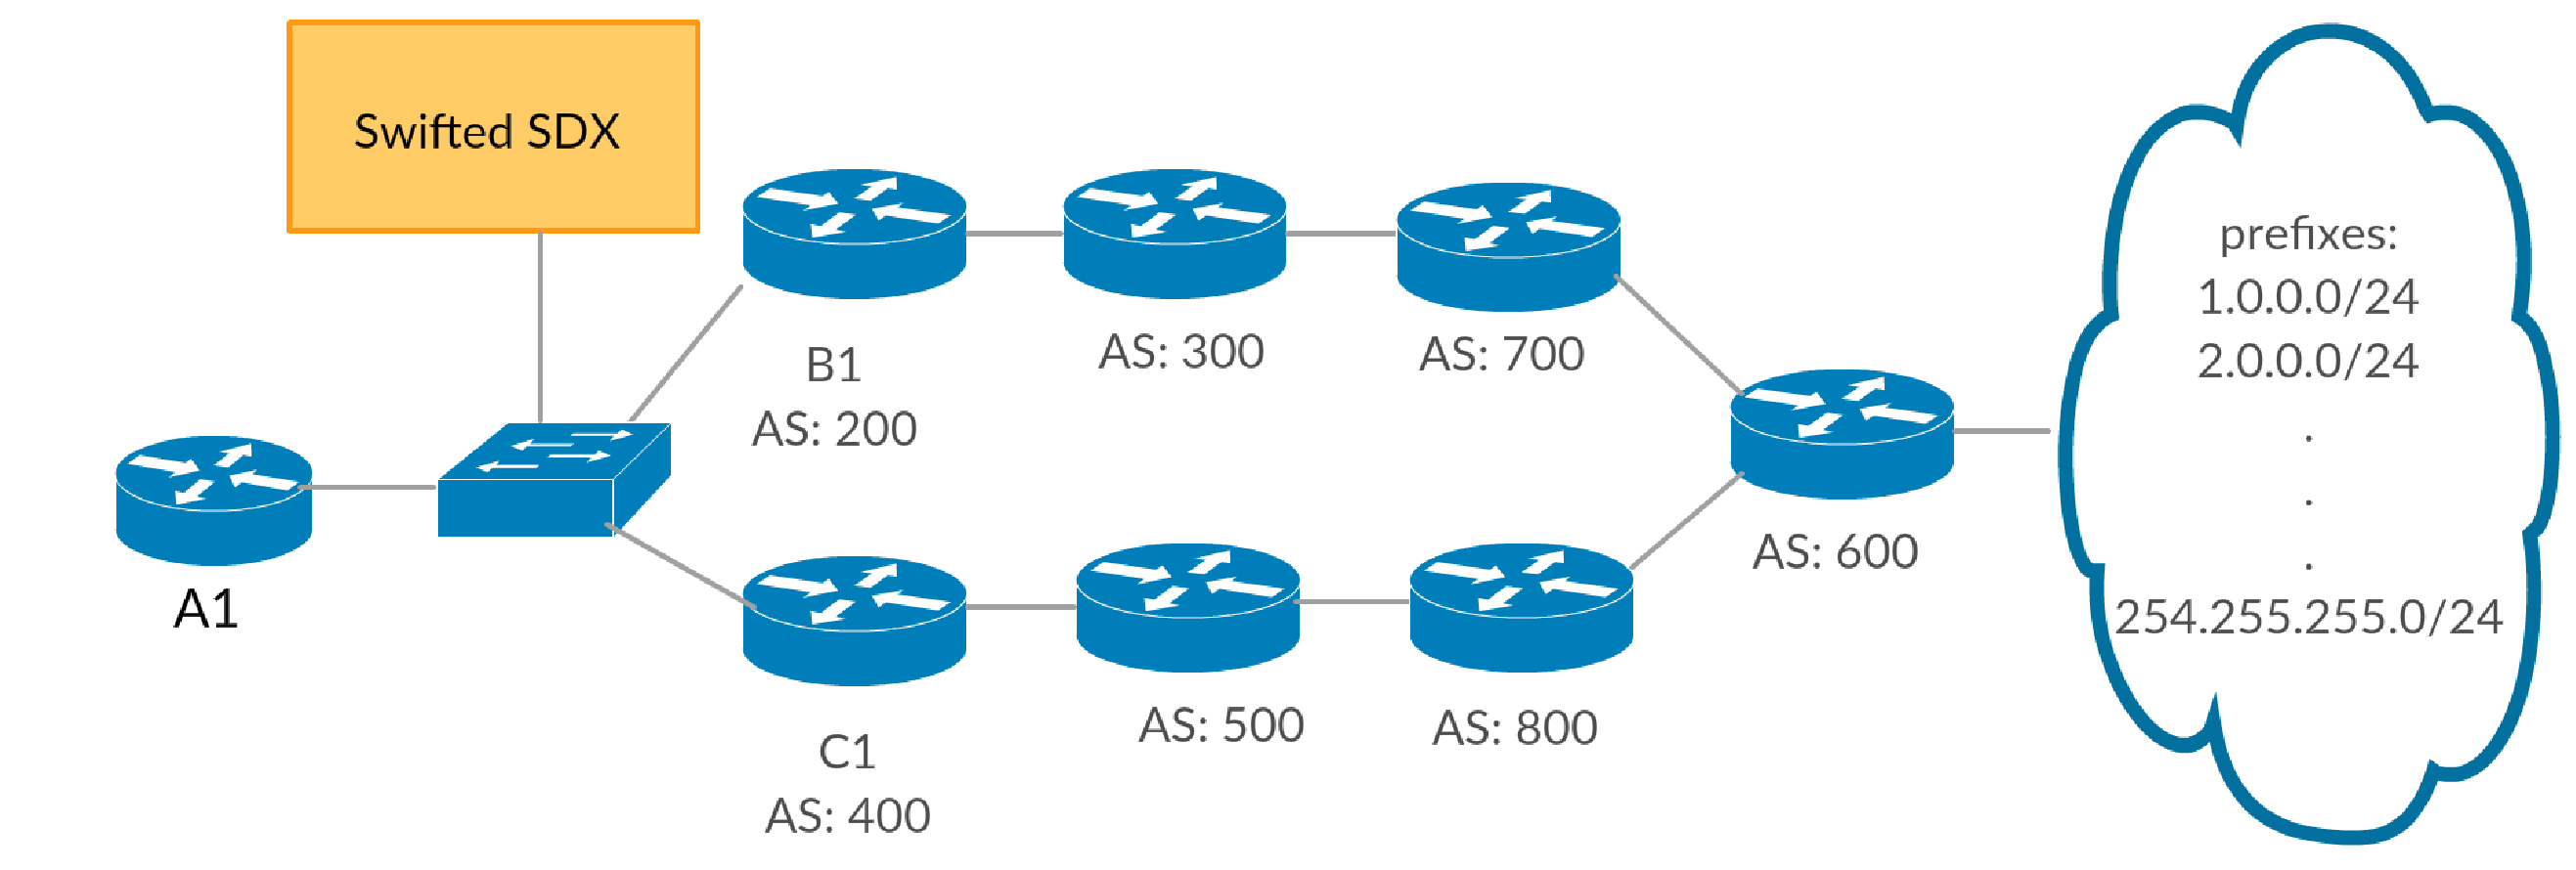
\includegraphics[scale = 0.24]{Figures/design_vmac_topology.pdf}
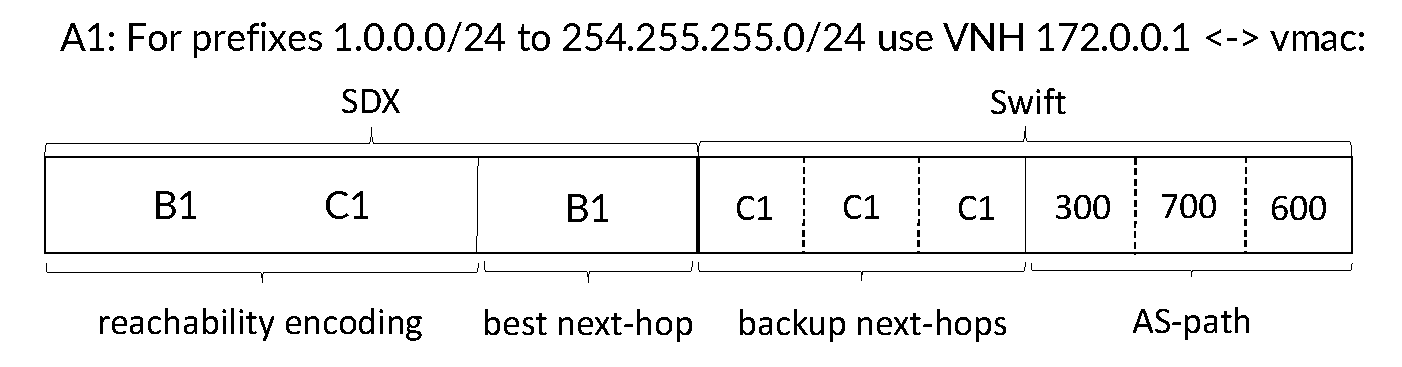
\includegraphics[scale = 0.35]{Figures/design_vmac_cropped.pdf}
\caption{example of the vmac in the iSDX with Swift}
\end{figure}

\newpage
